%
\begin{isabellebody}%
\def\isabellecontext{Misc}%
%
\isadelimtheory
%
\endisadelimtheory
%
\isatagtheory
\isacommand{theory}\isamarkupfalse%
\ Misc\isanewline
\isakeyword{imports}\ Base\isanewline
\isakeyword{begin}%
\endisatagtheory
{\isafoldtheory}%
%
\isadelimtheory
%
\endisadelimtheory
%
\isamarkupchapter{Miscellaneous tools \label{ch:tools}%
}
\isamarkuptrue%
%
\begin{isamarkuptext}%
Subsequently we describe various Isabelle related utilities, given
  in alphabetical order.%
\end{isamarkuptext}%
\isamarkuptrue%
%
\isamarkupsection{Displaying documents%
}
\isamarkuptrue%
%
\begin{isamarkuptext}%
The \indexdef{}{tool}{display}\hypertarget{tool.display}{\hyperlink{tool.display}{\mbox{\isa{\isatool{display}}}}} tool displays documents in DVI or PDF
  format:
\begin{ttbox}
Usage: isabelle display [OPTIONS] FILE

  Options are:
    -c           cleanup -- remove FILE after use

  Display document FILE (in DVI format).
\end{ttbox}

  \medskip The \verb|-c| option causes the input file to be
  removed after use.  The program for viewing \verb|dvi| files is
  determined by the \hyperlink{setting.DVI-VIEWER}{\mbox{\isa{\isatt{DVI{\isaliteral{5F}{\isacharunderscore}}VIEWER}}}} setting.%
\end{isamarkuptext}%
\isamarkuptrue%
%
\isamarkupsection{Viewing documentation \label{sec:tool-doc}%
}
\isamarkuptrue%
%
\begin{isamarkuptext}%
The \indexdef{}{tool}{doc}\hypertarget{tool.doc}{\hyperlink{tool.doc}{\mbox{\isa{\isatool{doc}}}}} tool displays online documentation:
\begin{ttbox}
Usage: isabelle doc [DOC]

  View Isabelle documentation DOC, or show list of available documents.
\end{ttbox}
  If called without arguments, it lists all available documents. Each
  line starts with an identifier, followed by a short description. Any
  of these identifiers may be specified as the first argument in order
  to have the corresponding document displayed.

  \medskip The \hyperlink{setting.ISABELLE-DOCS}{\mbox{\isa{\isatt{ISABELLE{\isaliteral{5F}{\isacharunderscore}}DOCS}}}} setting specifies the list of
  directories (separated by colons) to be scanned for documentations.
  The program for viewing \verb|dvi| files is determined by the
  \hyperlink{setting.DVI-VIEWER}{\mbox{\isa{\isatt{DVI{\isaliteral{5F}{\isacharunderscore}}VIEWER}}}} setting.%
\end{isamarkuptext}%
\isamarkuptrue%
%
\isamarkupsection{Shell commands within the settings environment \label{sec:tool-env}%
}
\isamarkuptrue%
%
\begin{isamarkuptext}%
The \indexdef{}{tool}{env}\hypertarget{tool.env}{\hyperlink{tool.env}{\mbox{\isa{\isatool{env}}}}} tool is a direct wrapper for the standard
  \verb|/usr/bin/env| command on POSIX systems, running within
  the Isabelle settings environment (\secref{sec:settings}).

  The command-line arguments are that of the underlying version of
  \verb|env|.  For example, the following invokes an instance of
  the GNU Bash shell within the Isabelle environment:
\begin{alltt}
  isabelle env bash
\end{alltt}%
\end{isamarkuptext}%
\isamarkuptrue%
%
\isamarkupsection{Getting logic images%
}
\isamarkuptrue%
%
\begin{isamarkuptext}%
The \indexdef{}{tool}{findlogics}\hypertarget{tool.findlogics}{\hyperlink{tool.findlogics}{\mbox{\isa{\isatool{findlogics}}}}} tool traverses all directories
  specified in \hyperlink{setting.ISABELLE-PATH}{\mbox{\isa{\isatt{ISABELLE{\isaliteral{5F}{\isacharunderscore}}PATH}}}}, looking for Isabelle logic
  images. Its usage is:
\begin{ttbox}
Usage: isabelle findlogics

  Collect heap file names from ISABELLE_PATH.
\end{ttbox}

  The base names of all files found on the path are printed --- sorted
  and with duplicates removed. Also note that lookup in \hyperlink{setting.ISABELLE-PATH}{\mbox{\isa{\isatt{ISABELLE{\isaliteral{5F}{\isacharunderscore}}PATH}}}} includes the current values of \hyperlink{setting.ML-SYSTEM}{\mbox{\isa{\isatt{ML{\isaliteral{5F}{\isacharunderscore}}SYSTEM}}}}
  and \hyperlink{setting.ML-PLATFORM}{\mbox{\isa{\isatt{ML{\isaliteral{5F}{\isacharunderscore}}PLATFORM}}}}. Thus switching to another ML compiler
  may change the set of logic images available.%
\end{isamarkuptext}%
\isamarkuptrue%
%
\isamarkupsection{Inspecting the settings environment \label{sec:tool-getenv}%
}
\isamarkuptrue%
%
\begin{isamarkuptext}%
The Isabelle settings environment --- as provided by the
  site-default and user-specific settings files --- can be inspected
  with the \indexdef{}{tool}{getenv}\hypertarget{tool.getenv}{\hyperlink{tool.getenv}{\mbox{\isa{\isatool{getenv}}}}} tool:
\begin{ttbox}
Usage: isabelle getenv [OPTIONS] [VARNAMES ...]

  Options are:
    -a           display complete environment
    -b           print values only (doesn't work for -a)
    -d FILE      dump complete environment to FILE
                 (null terminated entries)

  Get value of VARNAMES from the Isabelle settings.
\end{ttbox}

  With the \verb|-a| option, one may inspect the full process
  environment that Isabelle related programs are run in. This usually
  contains much more variables than are actually Isabelle settings.
  Normally, output is a list of lines of the form \isa{name}\verb|=|\isa{value}. The \verb|-b| option
  causes only the values to be printed.

  Option \verb|-d| produces a dump of the complete environment
  to the specified file.  Entries are terminated by the ASCII null
  character, i.e.\ the C string terminator.%
\end{isamarkuptext}%
\isamarkuptrue%
%
\isamarkupsubsubsection{Examples%
}
\isamarkuptrue%
%
\begin{isamarkuptext}%
Get the ML system name and the location where the compiler binaries
  are supposed to reside as follows:
\begin{ttbox}
isabelle getenv ML_SYSTEM ML_HOME
{\out ML_SYSTEM=polyml}
{\out ML_HOME=/usr/share/polyml/x86-linux}
\end{ttbox}

  The next one peeks at the output directory for Isabelle logic
  images:
\begin{ttbox}
isabelle getenv -b ISABELLE_OUTPUT
{\out /home/me/isabelle/heaps/polyml_x86-linux}
\end{ttbox}
  Here we have used the \verb|-b| option to suppress the
  \verb|ISABELLE_OUTPUT=| prefix.  The value above is what
  became of the following assignment in the default settings file:
\begin{ttbox}
ISABELLE_OUTPUT="\$ISABELLE_HOME_USER/heaps"
\end{ttbox}

  Note how the \hyperlink{setting.ML-IDENTIFIER}{\mbox{\isa{\isatt{ML{\isaliteral{5F}{\isacharunderscore}}IDENTIFIER}}}} value got appended
  automatically to each path component. This is a special feature of
  \hyperlink{setting.ISABELLE-OUTPUT}{\mbox{\isa{\isatt{ISABELLE{\isaliteral{5F}{\isacharunderscore}}OUTPUT}}}}.%
\end{isamarkuptext}%
\isamarkuptrue%
%
\isamarkupsection{Installing standalone Isabelle executables \label{sec:tool-install}%
}
\isamarkuptrue%
%
\begin{isamarkuptext}%
By default, the main Isabelle binaries (\hyperlink{executable.isabelle}{\mbox{\isa{\isatt{isabelle}}}} etc.)  are just run from their location within the
  distribution directory, probably indirectly by the shell through its
  \hyperlink{setting.PATH}{\mbox{\isa{\isatt{PATH}}}}.  Other schemes of installation are supported by the
  \indexdef{}{tool}{install}\hypertarget{tool.install}{\hyperlink{tool.install}{\mbox{\isa{\isatool{install}}}}} tool:
\begin{ttbox}
Usage: isabelle install [OPTIONS]

  Options are:
    -d DISTDIR   use DISTDIR as Isabelle distribution
                 (default ISABELLE_HOME)
    -p DIR       install standalone binaries in DIR

  Install Isabelle executables with absolute references to the current
  distribution directory.
\end{ttbox}

  The \verb|-d| option overrides the current Isabelle
  distribution directory as determined by \hyperlink{setting.ISABELLE-HOME}{\mbox{\isa{\isatt{ISABELLE{\isaliteral{5F}{\isacharunderscore}}HOME}}}}.

  The \verb|-p| option installs executable wrapper scripts for
  \hyperlink{executable.isabelle-process}{\mbox{\isa{\isatt{isabelle{\isaliteral{2D}{\isacharminus}}process}}}}, \hyperlink{executable.isabelle}{\mbox{\isa{\isatt{isabelle}}}},
  \hyperlink{executable.Isabelle}{\mbox{\isa{\isatt{Isabelle}}}}, containing proper absolute references to the
  Isabelle distribution directory.  A typical \verb|DIR|
  specification would be some directory expected to be in the shell's
  \hyperlink{setting.PATH}{\mbox{\isa{\isatt{PATH}}}}, such as \verb|/usr/local/bin|.  It is
  important to note that a plain manual copy of the original Isabelle
  executables does not work, since it disrupts the integrity of the
  Isabelle distribution.%
\end{isamarkuptext}%
\isamarkuptrue%
%
\isamarkupsection{Creating instances of the Isabelle logo%
}
\isamarkuptrue%
%
\begin{isamarkuptext}%
The \indexdef{}{tool}{logo}\hypertarget{tool.logo}{\hyperlink{tool.logo}{\mbox{\isa{\isatool{logo}}}}} tool creates any instance of the generic
  Isabelle logo as an Encapsuled Postscript file (EPS):
\begin{ttbox}
Usage: isabelle logo [OPTIONS] NAME

  Create instance NAME of the Isabelle logo (as EPS).

  Options are:
    -o OUTFILE   set output file (default determined from NAME)
    -q           quiet mode
\end{ttbox}
  You are encouraged to use this to create a derived logo for your
  Isabelle project.  For example, \hyperlink{tool.logo}{\mbox{\isa{\isatool{logo}}}}~\verb|Bali|
  creates \verb|isabelle_bali.eps|.%
\end{isamarkuptext}%
\isamarkuptrue%
%
\isamarkupsection{Isabelle wrapper for make \label{sec:tool-make}%
}
\isamarkuptrue%
%
\begin{isamarkuptext}%
The old \indexdef{}{tool}{make}\hypertarget{tool.make}{\hyperlink{tool.make}{\mbox{\isa{\isatool{make}}}}} tool is a very simple wrapper for
  ordinary Unix \hyperlink{executable.make}{\mbox{\isa{\isatt{make}}}}:
\begin{ttbox}
Usage: isabelle make [ARGS ...]

  Compile the logic in current directory using IsaMakefile.
  ARGS are directly passed to the system make program.
\end{ttbox}

  Note that the Isabelle settings environment is also active. Thus one
  may refer to its values within the \verb|IsaMakefile|, e.g.\
  \verb|$(ISABELLE_HOME)|. Furthermore, programs started from
  the make file also inherit this environment.%
\end{isamarkuptext}%
\isamarkuptrue%
%
\isamarkupsection{Creating Isabelle session directories
  \label{sec:tool-mkdir}%
}
\isamarkuptrue%
%
\begin{isamarkuptext}%
The old \indexdef{}{tool}{mkdir}\hypertarget{tool.mkdir}{\hyperlink{tool.mkdir}{\mbox{\isa{\isatool{mkdir}}}}} tool prepares Isabelle session
  source directories, including a sensible default setup of \verb|IsaMakefile|, \verb|ROOT.ML|, and a \verb|document|
  directory with a minimal \verb|root.tex| that is sufficient to
  print all theories of the session (in the order of appearance); see
  \secref{sec:tool-document} for further information on Isabelle
  document preparation.  The usage of \hyperlink{tool.mkdir}{\mbox{\isa{\isatool{mkdir}}}} is:

\begin{ttbox}
Usage: isabelle mkdir [OPTIONS] [LOGIC] NAME

  Options are:
    -I FILE      alternative IsaMakefile output
    -P           include parent logic target
    -b           setup build mode (session outputs heap image)
    -q           quiet mode

  Prepare session directory, including IsaMakefile and document source,
  with parent LOGIC (default ISABELLE_LOGIC=\$ISABELLE_LOGIC)
\end{ttbox}

  The \hyperlink{tool.mkdir}{\mbox{\isa{\isatool{mkdir}}}} tool is conservative in the sense that any
  existing \verb|IsaMakefile| etc.\ is left unchanged.  Thus it
  is safe to invoke it multiple times, although later runs may not
  have the desired effect.

  Note that \hyperlink{tool.mkdir}{\mbox{\isa{\isatool{mkdir}}}} is unable to change \verb|IsaMakefile|
  incrementally --- manual changes are required for multiple
  sub-sessions.  On order to get an initial working session, the only
  editing needed is to add appropriate \verb|use_thy| calls to the
  generated \verb|ROOT.ML| file.%
\end{isamarkuptext}%
\isamarkuptrue%
%
\isamarkupsubsubsection{Options%
}
\isamarkuptrue%
%
\begin{isamarkuptext}%
The \verb|-I| option specifies an alternative to \verb|IsaMakefile| for dependencies.  Note that ``\verb|-|'' refers
  to \emph{stdout}, i.e.\ ``\verb|-I-|'' provides an easy way
  to peek at \hyperlink{tool.mkdir}{\mbox{\isa{\isatool{mkdir}}}}'s idea of \hyperlink{tool.make}{\mbox{\isa{\isatool{make}}}} setup required for
  some particular of Isabelle session.

  \medskip The \verb|-P| option includes a target for the
  parent \verb|LOGIC| session in the generated \verb|IsaMakefile|.  The corresponding sources are assumed to be located
  within the Isabelle distribution.

  \medskip The \verb|-b| option sets up the current directory
  as the base for a new session that provides an actual logic image,
  as opposed to one that only runs several theories based on an
  existing image.  Note that in the latter case, everything except
  \verb|IsaMakefile| would be placed into a separate directory
  \verb|NAME|, rather than the current one.  See
  \secref{sec:tool-usedir} for further information on \emph{build
  mode} vs.\ \emph{example mode} of \hyperlink{tool.usedir}{\mbox{\isa{\isatool{usedir}}}}.

  \medskip The \verb|-q| option enables quiet mode, suppressing
  further notes on how to proceed.%
\end{isamarkuptext}%
\isamarkuptrue%
%
\isamarkupsection{Printing documents%
}
\isamarkuptrue%
%
\begin{isamarkuptext}%
The \indexdef{}{tool}{print}\hypertarget{tool.print}{\hyperlink{tool.print}{\mbox{\isa{\isatool{print}}}}} tool prints documents:
\begin{ttbox}
Usage: isabelle print [OPTIONS] FILE

  Options are:
    -c           cleanup -- remove FILE after use

  Print document FILE.
\end{ttbox}

  The \verb|-c| option causes the input file to be removed
  after use.  The printer spool command is determined by the \hyperlink{setting.PRINT-COMMAND}{\mbox{\isa{\isatt{PRINT{\isaliteral{5F}{\isacharunderscore}}COMMAND}}}} setting.%
\end{isamarkuptext}%
\isamarkuptrue%
%
\isamarkupsection{Remove awkward symbol names from theory sources%
}
\isamarkuptrue%
%
\begin{isamarkuptext}%
The \indexdef{}{tool}{unsymbolize}\hypertarget{tool.unsymbolize}{\hyperlink{tool.unsymbolize}{\mbox{\isa{\isatool{unsymbolize}}}}} tool tunes Isabelle theory sources to
  improve readability for plain ASCII output (e.g.\ in email
  communication).  Most notably, \hyperlink{tool.unsymbolize}{\mbox{\isa{\isatool{unsymbolize}}}} replaces awkward
  arrow symbols such as \verb|\|\verb|<Longrightarrow>|
  by \verb|==>|.
\begin{ttbox}
Usage: isabelle unsymbolize [FILES|DIRS...]

  Recursively find .thy/.ML files, removing unreadable symbol names.
  Note: this is an ad-hoc script; there is no systematic way to replace
  symbols independently of the inner syntax of a theory!

  Renames old versions of FILES by appending "~~".
\end{ttbox}%
\end{isamarkuptext}%
\isamarkuptrue%
%
\isamarkupsection{Running Isabelle sessions \label{sec:tool-usedir}%
}
\isamarkuptrue%
%
\begin{isamarkuptext}%
The old \indexdef{}{tool}{usedir}\hypertarget{tool.usedir}{\hyperlink{tool.usedir}{\mbox{\isa{\isatool{usedir}}}}} tool builds object-logic images, or
  runs example sessions based on existing logics. Its usage is:
\begin{ttbox}
Usage: isabelle usedir [OPTIONS] LOGIC NAME

  Options are:
    -C BOOL      copy existing document directory to -D PATH (default true)
    -D PATH      dump generated document sources into PATH
    -M MAX       multithreading: maximum number of worker threads (default 1)
    -P PATH      set path for remote theory browsing information
    -Q INT       set threshold for sub-proof parallelization (default 50)
    -T LEVEL     multithreading: trace level (default 0)
    -V VARIANT   declare alternative document VARIANT
    -b           build mode (output heap image, using current dir)
    -d FORMAT    build document as FORMAT (default false)
    -f NAME      use ML file NAME (default ROOT.ML)
    -g BOOL      generate session graph image for document (default false)
    -i BOOL      generate theory browser information (default false)
    -m MODE      add print mode for output
    -p LEVEL     set level of detail for proof objects (default 0)
    -q LEVEL     set level of parallel proof checking (default 1)
    -r           reset session path
    -s NAME      override session NAME
    -t BOOL      internal session timing (default false)
    -v BOOL      be verbose (default false)

  Build object-logic or run examples. Also creates browsing
  information (HTML etc.) according to settings.

  ISABELLE_USEDIR_OPTIONS=...

  ML_PLATFORM=...
  ML_HOME=...
  ML_SYSTEM=...
  ML_OPTIONS=...
\end{ttbox}

  Note that the value of the \indexref{}{setting}{ISABELLE\_USEDIR\_OPTIONS}\hyperlink{setting.ISABELLE-USEDIR-OPTIONS}{\mbox{\isa{\isatt{ISABELLE{\isaliteral{5F}{\isacharunderscore}}USEDIR{\isaliteral{5F}{\isacharunderscore}}OPTIONS}}}}
  setting is implicitly prefixed to \emph{any} \hyperlink{tool.usedir}{\mbox{\isa{\isatool{usedir}}}}
  call. Since the \verb|IsaMakefile|s of all object-logics
  distributed with Isabelle just invoke \hyperlink{tool.usedir}{\mbox{\isa{\isatool{usedir}}}} for the real
  work, one may control compilation options globally via above
  variable. In particular, generation of \rmindex{HTML} browsing
  information and document preparation is controlled here.%
\end{isamarkuptext}%
\isamarkuptrue%
%
\isamarkupsubsubsection{Options%
}
\isamarkuptrue%
%
\begin{isamarkuptext}%
Basically, there are two different modes of operation: \emph{build
  mode} (enabled through the \verb|-b| option) and
  \emph{example mode} (default).

  Calling \hyperlink{tool.usedir}{\mbox{\isa{\isatool{usedir}}}} with \verb|-b| runs \hyperlink{executable.isabelle-process}{\mbox{\isa{\isatt{isabelle{\isaliteral{2D}{\isacharminus}}process}}}} with input image \verb|LOGIC| and output to
  \verb|NAME|, as provided on the command line. This will be a
  batch session, running \verb|ROOT.ML| from the current
  directory and then quitting.  It is assumed that \verb|ROOT.ML|
  contains all ML commands required to build the logic.

  In example mode, \hyperlink{tool.usedir}{\mbox{\isa{\isatool{usedir}}}} runs a read-only session of
  \verb|LOGIC| and automatically runs \verb|ROOT.ML| from
  within directory \verb|NAME|.  It assumes that this file
  contains appropriate ML commands to run the desired examples.

  \medskip The \verb|-i| option controls theory browser data
  generation. It may be explicitly turned on or off --- as usual, the
  last occurrence of \verb|-i| on the command line wins.

  The \verb|-P| option specifies a path (or actual URL) to be
  prefixed to any \emph{non-local} reference of existing theories.
  Thus user sessions may easily link to existing Isabelle libraries
  already present on the WWW.

  The \verb|-m| options specifies additional print modes to be
  activated temporarily while the session is processed.

  \medskip The \verb|-d| option controls document preparation.
  Valid arguments are \verb|false| (do not prepare any document;
  this is default), or any of \verb|dvi|, \verb|dvi.gz|,
  \verb|ps|, \verb|ps.gz|, \verb|pdf|.  The logic
  session has to provide a properly setup \verb|document|
  directory.  See \secref{sec:tool-document} and
  \secref{sec:tool-latex} for more details.

  \medskip The \verb|-V| option declares alternative document
  variants, consisting of name/tags pairs (cf.\ options \verb|-n| and \verb|-t| of \indexref{}{tool}{document}\hyperlink{tool.document}{\mbox{\isa{\isatool{document}}}}).  The standard
  document is equivalent to ``\verb|document=theory,proof,ML|'', which means that all theory begin/end
  commands, proof body texts, and ML code will be presented
  faithfully.

  An alternative variant ``\verb|outline=/proof/ML|'' would
  fold proof and ML parts, replacing the original text by a short
  place-holder.  The form ``\isa{name}\verb|=-|,'' means to
  remove document \isa{name} from the list of variants to be
  processed.  Any number of \verb|-V| options may be given;
  later declarations have precedence over earlier ones.

  Some document variant \isa{name} may use an alternative {\LaTeX}
  entry point called \verb|document/root_|\isa{{\isaliteral{22}{\isachardoublequote}}name{\isaliteral{22}{\isachardoublequote}}}\verb|.tex| if that file exists; otherwise the common
  \verb|document/root.tex| is used.

  \medskip The \verb|-g| option produces images of the theory
  dependency graph (cf.\ \secref{sec:browse}) for inclusion in the
  generated document, both as \verb|session_graph.eps| and
  \verb|session_graph.pdf| at the same time.  To include this in
  the final {\LaTeX} document one could say \verb|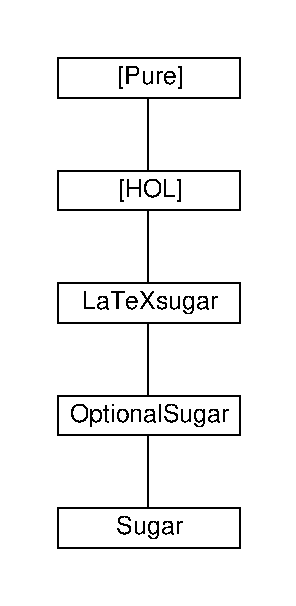
\includegraphics{session_graph}| in \verb|document/root.tex| (omitting the file-name extension enables
  {\LaTeX} to select to correct version, either for the DVI or PDF
  output path).

  \medskip The \verb|-D| option causes the generated document
  sources to be dumped at location \verb|PATH|; this path is
  relative to the session's main directory.  If the \verb|-C|
  option is true, this will include a copy of an existing \verb|document| directory as provided by the user.  For example, \hyperlink{tool.usedir}{\mbox{\isa{\isatool{usedir}}}}~\verb|-D generated HOL Foo| produces a complete set
  of document sources at \verb|Foo/generated|.  Subsequent
  invocation of \hyperlink{tool.document}{\mbox{\isa{\isatool{document}}}}~\verb|Foo/generated| (see also
  \secref{sec:tool-document}) will process the final result
  independently of an Isabelle job.  This decoupled mode of operation
  facilitates debugging of serious {\LaTeX} errors, for example.

  \medskip The \verb|-p| option determines the level of detail
  for internal proof objects, see also the \emph{Isabelle Reference
  Manual}~\cite{isabelle-ref}.

  \medskip The \verb|-q| option specifies the level of parallel
  proof checking: \verb|0| no proofs, \verb|1| toplevel
  proofs (default), \verb|2| toplevel and nested Isar proofs.
  The option \verb|-Q| specifies a threshold for \verb|-q2|: nested proofs are only parallelized when the current number
  of forked proofs falls below the given value (default 50),
  multiplied by the number of worker threads (see option \verb|-M|).

  \medskip The \verb|-t| option produces a more detailed
  internal timing report of the session.

  \medskip The \verb|-v| option causes additional information
  to be printed while running the session, notably the location of
  prepared documents.

  \medskip The \verb|-M| option specifies the maximum number of
  parallel worker threads used for processing independent tasks when
  checking theory sources (multithreading only works on suitable ML
  platforms).  The special value of \verb|0| or \verb|max|
  refers to the number of actual CPU cores of the underlying machine,
  which is a good starting point for optimal performance tuning.  The
  \verb|-T| option determines the level of detail in tracing
  output concerning the internal locking and scheduling in
  multithreaded operation.  This may be helpful in isolating
  performance bottle-necks, e.g.\ due to excessive wait states when
  locking critical code sections.

  \medskip Any \hyperlink{tool.usedir}{\mbox{\isa{\isatool{usedir}}}} session is named by some \emph{session
  identifier}. These accumulate, documenting the way sessions depend
  on others. For example, consider \verb|Pure/FOL/ex|, which
  refers to the examples of FOL, which in turn is built upon Pure.

  The current session's identifier is by default just the base name of
  the \verb|LOGIC| argument (in build mode), or of the \verb|NAME| argument (in example mode). This may be overridden explicitly
  via the \verb|-s| option.%
\end{isamarkuptext}%
\isamarkuptrue%
%
\isamarkupsection{Output the version identifier of the Isabelle distribution%
}
\isamarkuptrue%
%
\begin{isamarkuptext}%
The \indexdef{}{tool}{version}\hypertarget{tool.version}{\hyperlink{tool.version}{\mbox{\isa{\isatool{version}}}}} tool displays Isabelle version information:
\begin{ttbox}
Usage: isabelle version [OPTIONS]

  Options are:
    -i           short identification (derived from Mercurial id)

  Display Isabelle version information.
\end{ttbox}

  \medskip The default is to output the full version string of the
  Isabelle distribution, e.g.\ ``\verb|Isabelle2012: May 2012|.

  The \verb|-i| option produces a short identification derived
  from the Mercurial id of the \hyperlink{setting.ISABELLE-HOME}{\mbox{\isa{\isatt{ISABELLE{\isaliteral{5F}{\isacharunderscore}}HOME}}}} directory.%
\end{isamarkuptext}%
\isamarkuptrue%
%
\isamarkupsection{Convert XML to YXML%
}
\isamarkuptrue%
%
\begin{isamarkuptext}%
The \indexdef{}{tool}{yxml}\hypertarget{tool.yxml}{\hyperlink{tool.yxml}{\mbox{\isa{\isatool{yxml}}}}} tool converts a standard XML document (stdin)
  to the much simpler and more efficient YXML format of Isabelle
  (stdout).  The YXML format is defined as follows.

  \begin{enumerate}

  \item The encoding is always UTF-8.

  \item Body text is represented verbatim (no escaping, no special
  treatment of white space, no named entities, no CDATA chunks, no
  comments).

  \item Markup elements are represented via ASCII control characters
  \isa{{\isaliteral{22}{\isachardoublequote}}\isaliteral{5C3C5E626F6C643E}{}\isactrlbold X\ {\isaliteral{3D}{\isacharequal}}\ {\isadigit{5}}{\isaliteral{22}{\isachardoublequote}}} and \isa{{\isaliteral{22}{\isachardoublequote}}\isaliteral{5C3C5E626F6C643E}{}\isactrlbold Y\ {\isaliteral{3D}{\isacharequal}}\ {\isadigit{6}}{\isaliteral{22}{\isachardoublequote}}} as follows:

  \begin{tabular}{ll}
    XML & YXML \\\hline
    \verb|<|\isa{{\isaliteral{22}{\isachardoublequote}}name\ attribute{\isaliteral{22}{\isachardoublequote}}}\verb|=|\isa{{\isaliteral{22}{\isachardoublequote}}value\ {\isaliteral{5C3C646F74733E}{\isasymdots}}{\isaliteral{22}{\isachardoublequote}}}\verb|>| &
    \isa{{\isaliteral{22}{\isachardoublequote}}\isaliteral{5C3C5E626F6C643E}{}\isactrlbold X\isaliteral{5C3C5E626F6C643E}{}\isactrlbold Yname\isaliteral{5C3C5E626F6C643E}{}\isactrlbold Yattribute{\isaliteral{22}{\isachardoublequote}}}\verb|=|\isa{{\isaliteral{22}{\isachardoublequote}}value{\isaliteral{5C3C646F74733E}{\isasymdots}}\isaliteral{5C3C5E626F6C643E}{}\isactrlbold X{\isaliteral{22}{\isachardoublequote}}} \\
    \verb|</|\isa{name}\verb|>| & \isa{{\isaliteral{22}{\isachardoublequote}}\isaliteral{5C3C5E626F6C643E}{}\isactrlbold X\isaliteral{5C3C5E626F6C643E}{}\isactrlbold Y\isaliteral{5C3C5E626F6C643E}{}\isactrlbold X{\isaliteral{22}{\isachardoublequote}}} \\
  \end{tabular}

  There is no special case for empty body text, i.e.\ \verb|<foo/>| is treated like \verb|<foo></foo>|.  Also note that
  \isa{{\isaliteral{22}{\isachardoublequote}}\isaliteral{5C3C5E626F6C643E}{}\isactrlbold X{\isaliteral{22}{\isachardoublequote}}} and \isa{{\isaliteral{22}{\isachardoublequote}}\isaliteral{5C3C5E626F6C643E}{}\isactrlbold Y{\isaliteral{22}{\isachardoublequote}}} may never occur in
  well-formed XML documents.

  \end{enumerate}

  Parsing YXML is pretty straight-forward: split the text into chunks
  separated by \isa{{\isaliteral{22}{\isachardoublequote}}\isaliteral{5C3C5E626F6C643E}{}\isactrlbold X{\isaliteral{22}{\isachardoublequote}}}, then split each chunk into
  sub-chunks separated by \isa{{\isaliteral{22}{\isachardoublequote}}\isaliteral{5C3C5E626F6C643E}{}\isactrlbold Y{\isaliteral{22}{\isachardoublequote}}}.  Markup chunks start
  with an empty sub-chunk, and a second empty sub-chunk indicates
  close of an element.  Any other non-empty chunk consists of plain
  text.  For example, see \verb|~~/src/Pure/PIDE/yxml.ML| or
  \verb|~~/src/Pure/PIDE/yxml.scala|.

  YXML documents may be detected quickly by checking that the first
  two characters are \isa{{\isaliteral{22}{\isachardoublequote}}\isaliteral{5C3C5E626F6C643E}{}\isactrlbold X\isaliteral{5C3C5E626F6C643E}{}\isactrlbold Y{\isaliteral{22}{\isachardoublequote}}}.%
\end{isamarkuptext}%
\isamarkuptrue%
%
\isadelimtheory
%
\endisadelimtheory
%
\isatagtheory
\isacommand{end}\isamarkupfalse%
%
\endisatagtheory
{\isafoldtheory}%
%
\isadelimtheory
%
\endisadelimtheory
\end{isabellebody}%
%%% Local Variables:
%%% mode: latex
%%% TeX-master: "root"
%%% End:
